\section{Results}
\label{sec:result}

Our algorithm is tested on a variety of 3D shapes.
We visualize the discrete matches using the similar color as the corresponding symmetry parts.

We first show experimental results on clean manifold meshes, which are not corrupted with noise, and are complete.
For such models, our algorithm provides good segmentation for the partial matching, and we reliably obtain perfect results (e.g. Figure~\ref{fig:Eager} and~\ref{fig:Tiger}).

\begin{figure}[t]
\centering
  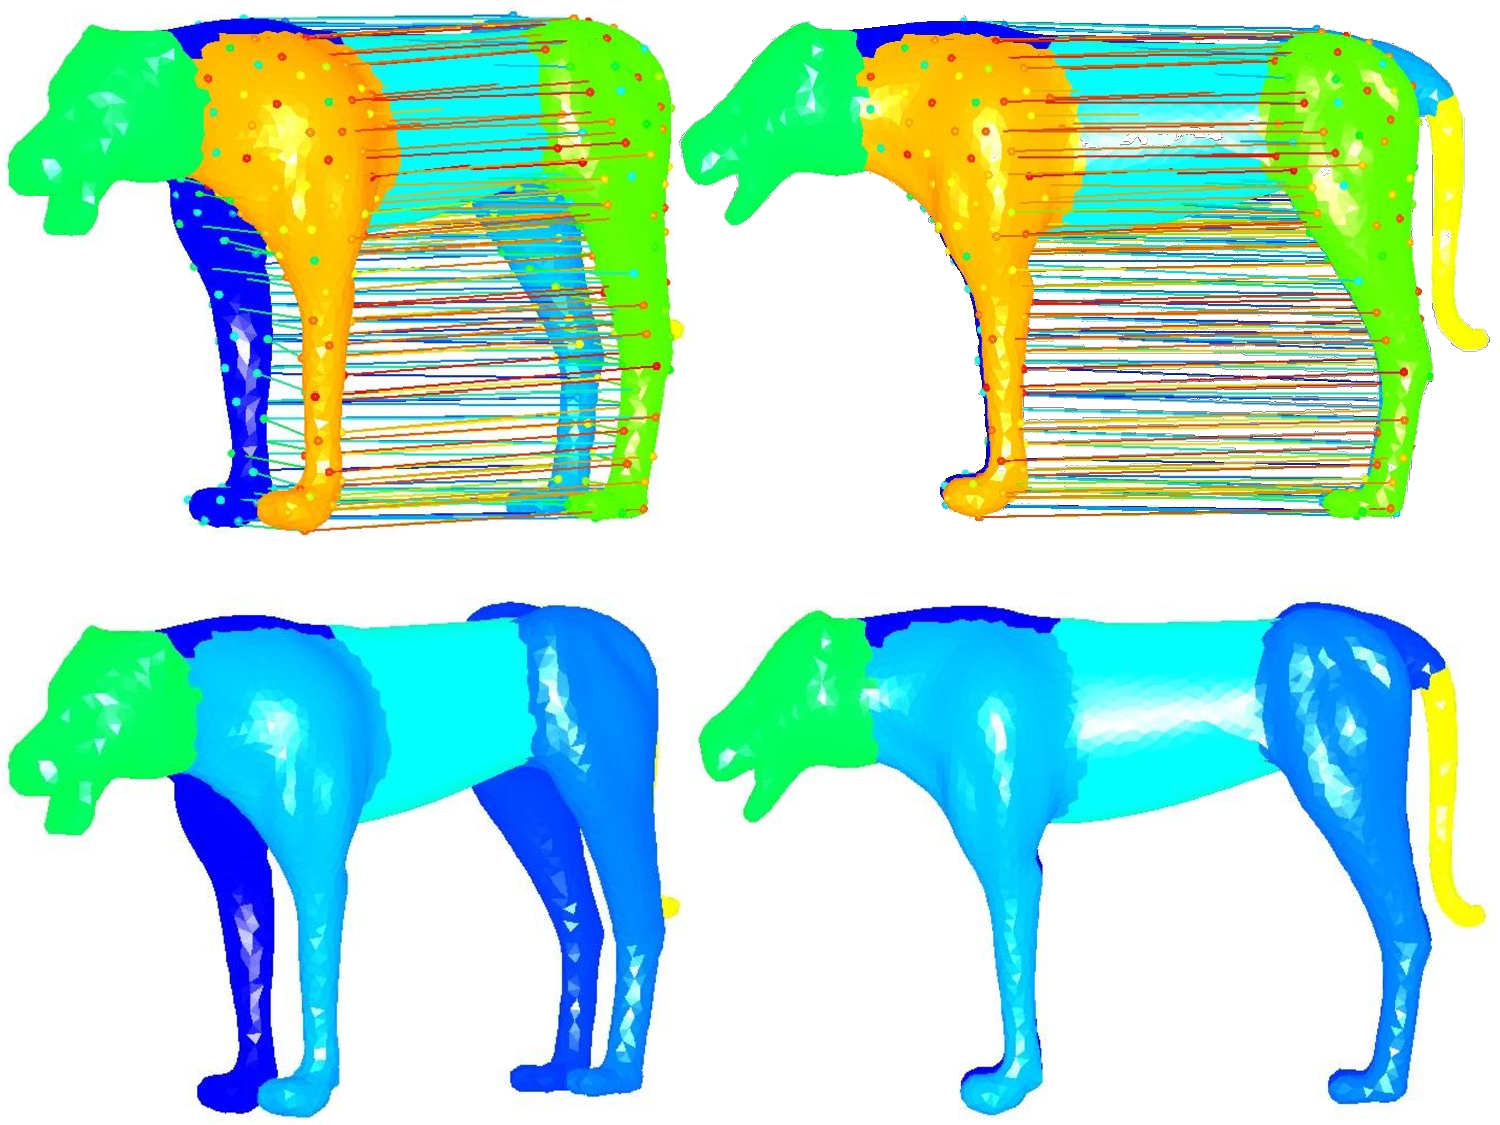
\includegraphics[width=0.99\linewidth]{figures/chetah.pdf}
  \caption{The four legs of Chetah could be detected as one symmetric region at the current configuration $c=0.2/n$ and $m=100 \times n$.
  It is mainly resulting from the large similarity of four legs.}
\label{fig:Tiger}
\end{figure}

As our algorithm works on the segmentation, uniform sampling, and clustering, the matching results do not depend on the representation and tessellation of the shapes.
Figure~\ref{fig:Point} demonstrates that our algorithm performs very well on the shape in the point set form.
Simultaneously, it proves that our algorithm is insensitive to the shape remeshing, as the left and right regions of Dinosaur are in large different resolutions.

\begin{figure}[t]
\centering
  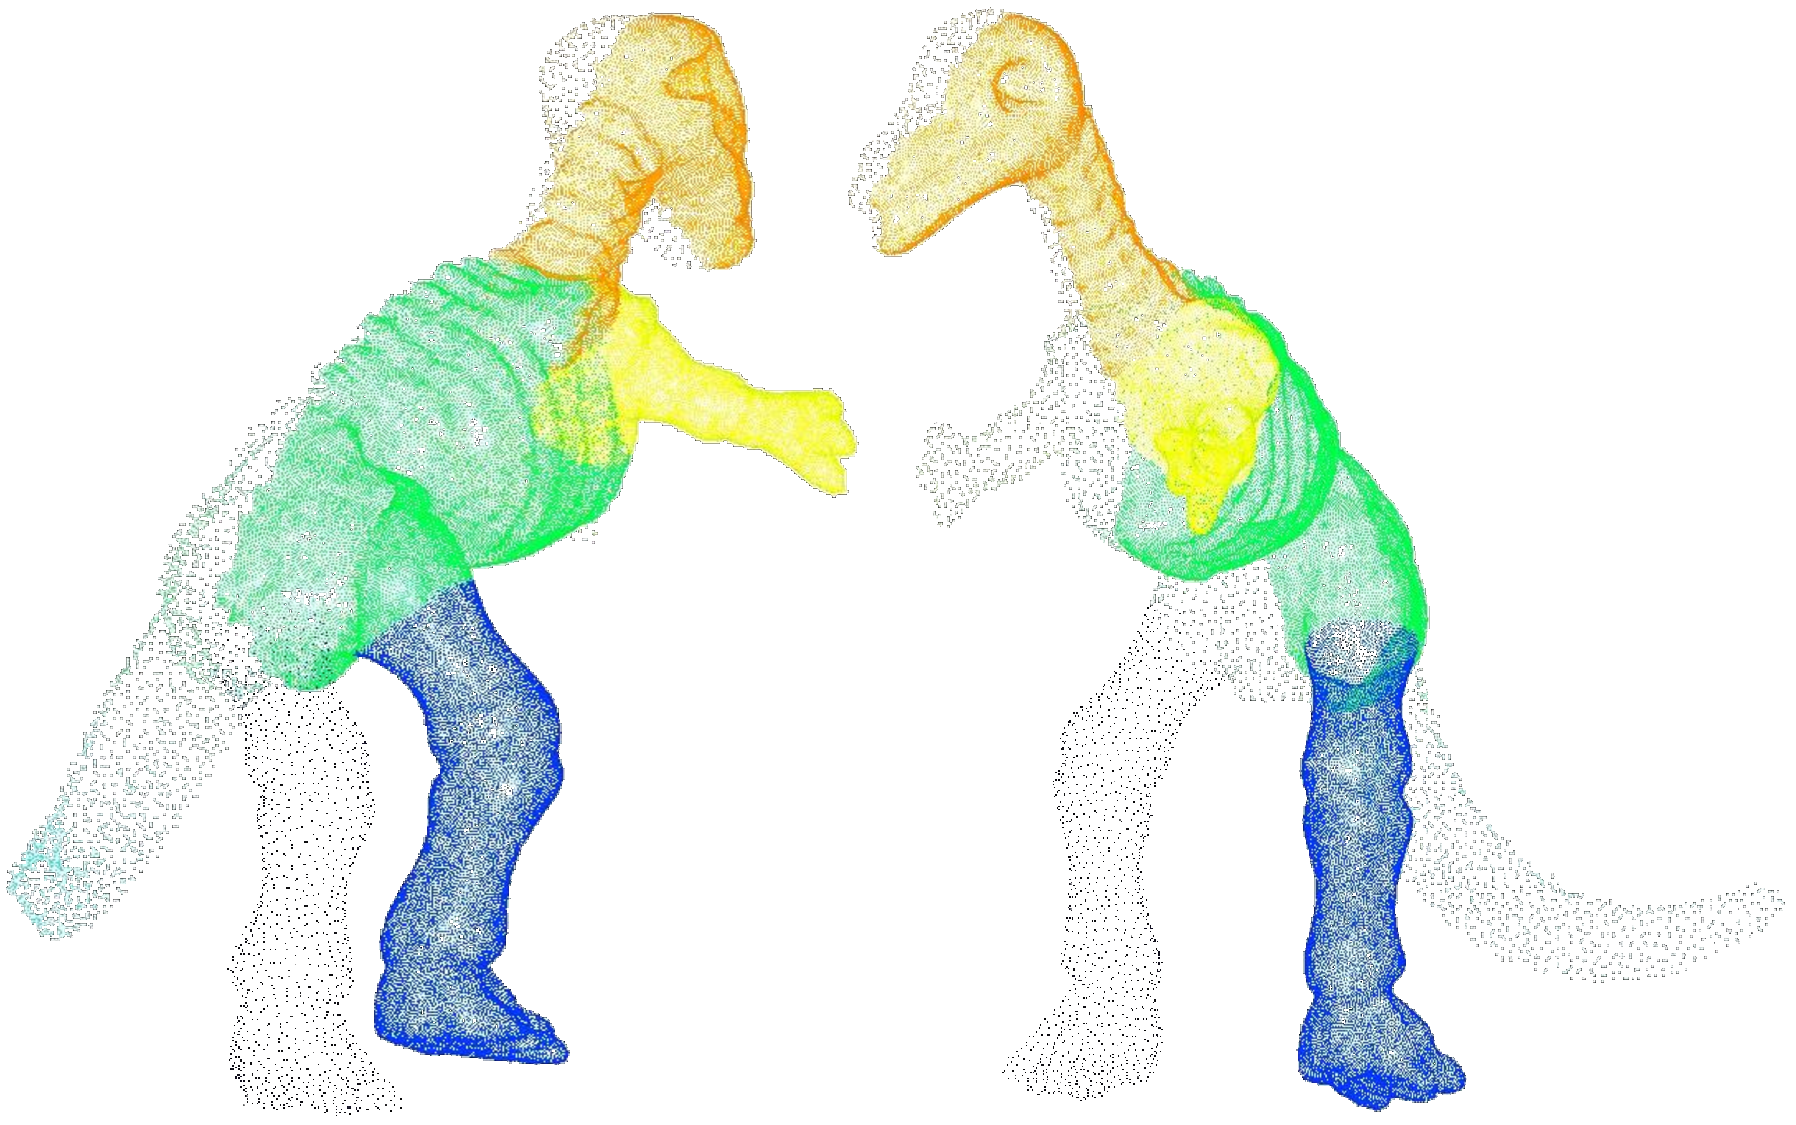
\includegraphics[width=0.99\linewidth]{figures/dinosaur.pdf}
  \caption{The symmetry detection of point set Dinosaur with different resolutions in the left and right regions. The left and right legs are detected as the symmetric.}
\label{fig:Point}
\end{figure}

Figure~\ref{fig:Gargoyl} shows an example using the three different symmetry group composed of reflection, rotation, and translation.
The symmetry is detected in coarse-to-fine steps based on the hierarchical segmentation.
In the coarse level, all major reflection symmetries are faithfully recovered.
While in the fine level, most rotation and translation symmetries are detected.
Note that, the example is clearly claimed as the failure case in the STAR algorithm~\cite{berner2011}.

We use another example on the complete and non-complete Armidillo (Figure~\ref{fig:Arm}) to demonstrate the robustness of our algorithm.
Both on the complete and non-complete cases, the algorithm computes a global reflectional plane based on all final correspondences.
Experiments show that the plane is almost totally same in the both cases.

\begin{figure}[t]
\centering
  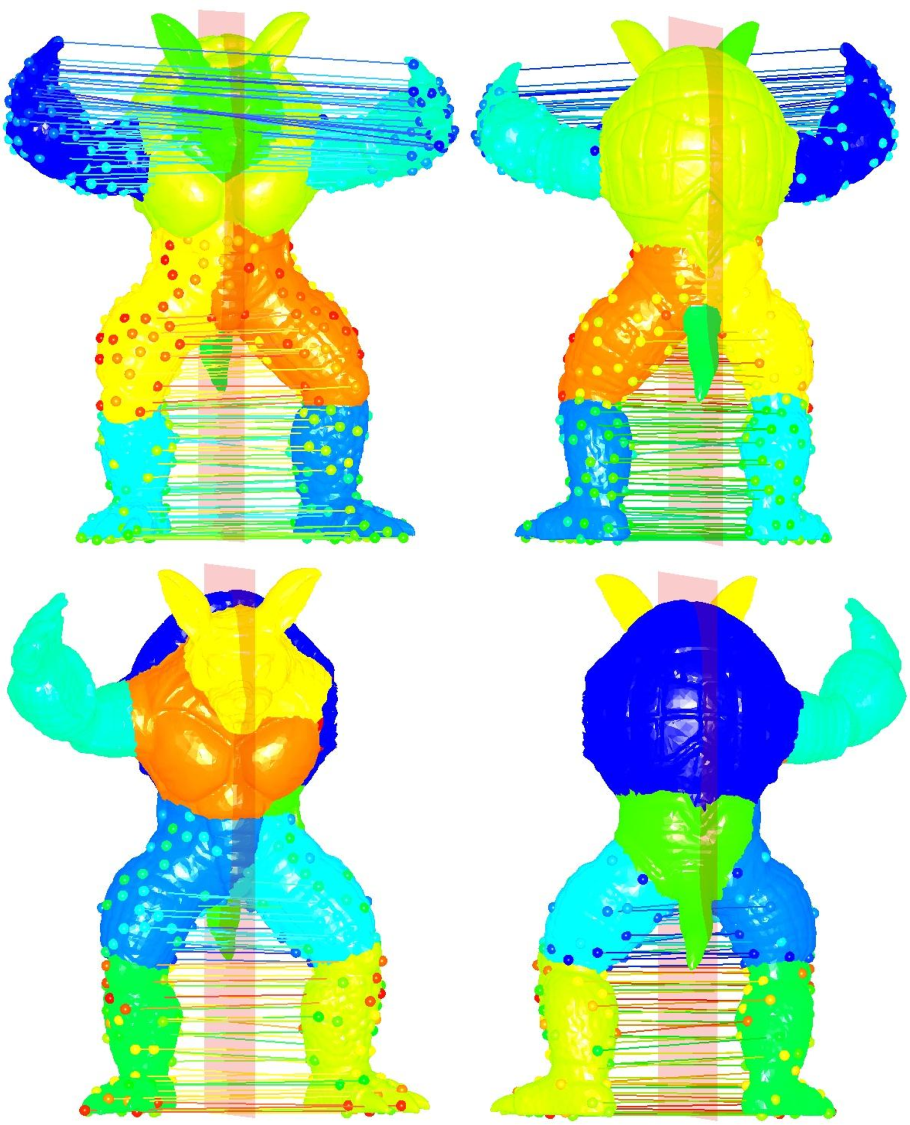
\includegraphics[width=0.99\linewidth]{figures/Armadillo.pdf}
  \caption{The global reflectional planes are almost totally same, which are computed from both the complete and non-complete Armadillo shapes.}
\label{fig:Arm}
\end{figure}

At last, we use the iterative segmentation and symmetry detection steps to improve the output results, on both the shape segmentation and symmetry detection. 
Firstly, this shape is particularly reasonable segmented since it is so complex that the segmentation algorithm~\cite{lai2009} is difficult to handle.
Beyond the segmentation, the symmetry is detected as before. Then, using the detected reflectional symmetry information, we further improve the segmentation.
The Figure~\ref{fig:iteration} shows the initial segmentation and symmetry detection, and the refined results after two iteration.

\begin{figure}[t]
\centering
  %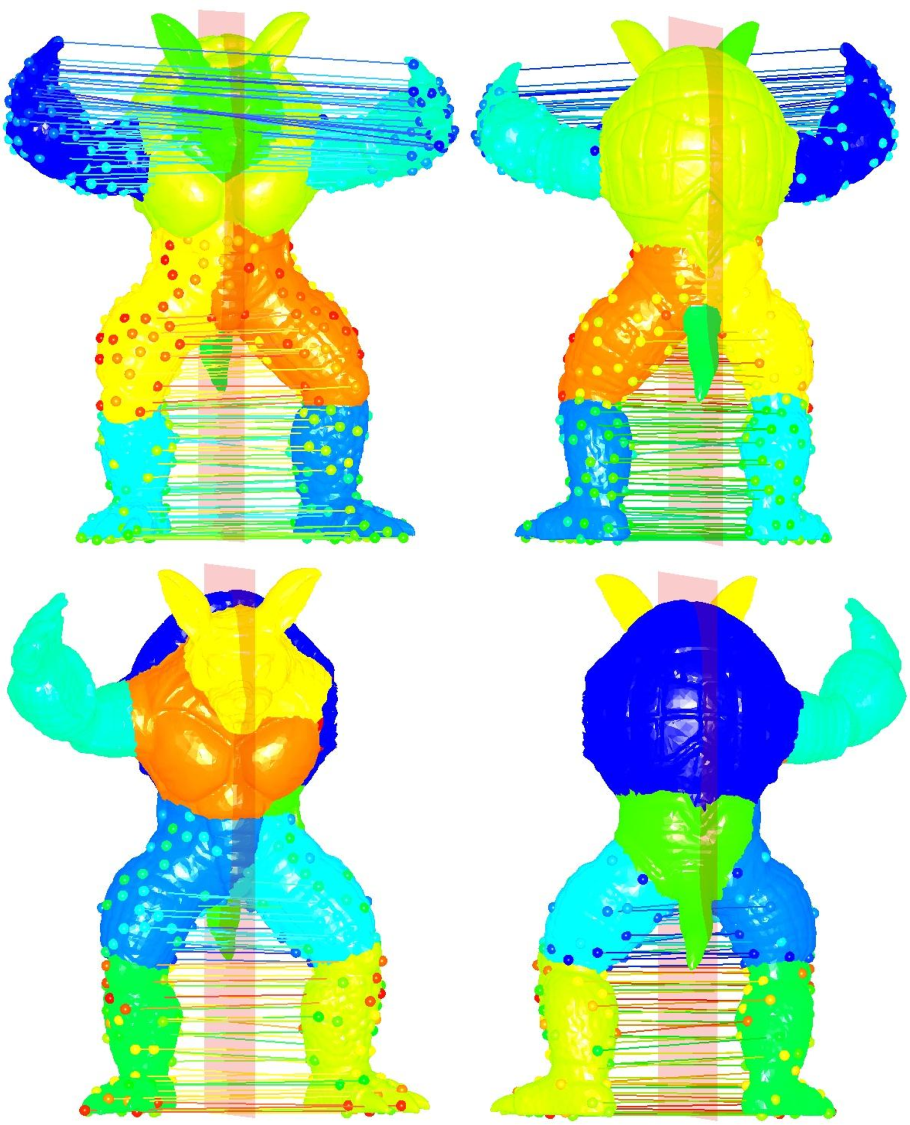
\includegraphics[width=0.99\linewidth]{figures/Armadillo.pdf}
  \caption{The iterative segmentation and symmetry detection. Top: the initial results, below: the results after two iteration.}
\label{fig:iteration}
\end{figure}

The performance data of Table~\ref{tab:timing} indicates how the computation on the symmetry of 3d shapes.
From the table, it is easy to note that the partial matching time is higher as the more segmentation, but less sensitive to vertex number of each shape.
The reason is that the sampling point is the key issue to the time complexity, and it is linearly dependent on the segmentation parts number in the paper.

\begin{table*}
\centering
\begin{tabular}{l|r|r|r|r|r}
Model
& Vertices
& Parts number
& Segmentation
& Partial matching
& Correspondences clustering \\
\hline
%%%RRM Use captial letter for all model names
Armadillo  & 172,974  & 9 &  1.6s   & 959.0s & 7.8s \\
Chetah     &   5,000  & 7 &  0.2s   & 588.2s & 5.2s  \\
Dinosaur   &  69,215  & 7 &  3.2s   & 522.7s & 5.1s   \\
Eager      &  14,618  & 6 &  0.5s   & 403.1s & 3.2s \\
Gargoyl    & 250,003  & 6 &  3.6s   & 448.9s & 3.9s  \\
\hline
\end{tabular}
\caption{Timing for our algorithm: automatic meaningful segmentation, partial matching of each part,
and clustering the correspondences, using a 1.6GHz Intel Core i7CPU laptop with 4GB of RAM.
}
\label{tab:timing}
\end{table*} 